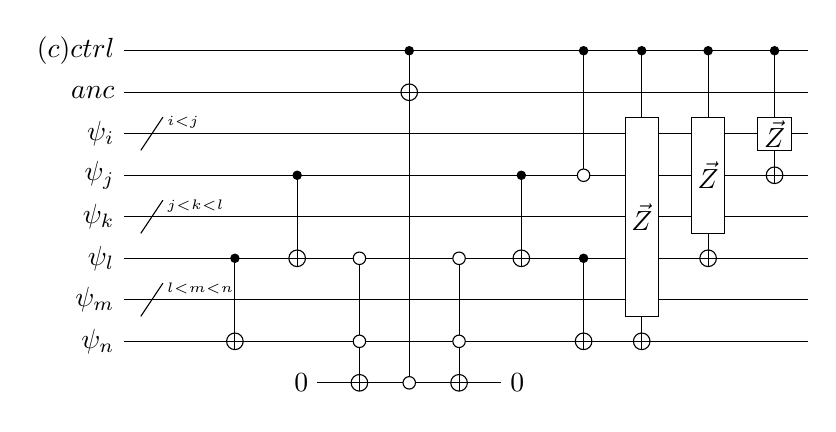
\begin{tikzpicture}[scale=1.000000,x=1pt,y=1pt]
\filldraw[color=white] (0.000000, -7.500000) rectangle (247.000000, 127.500000);
% Drawing wires
% Line 1: ctrl W \text{(c) }ctrl
\draw[color=black] (0.000000,120.000000) -- (247.000000,120.000000);
\draw[color=black] (0.000000,120.000000) node[left] {$\text{(c) }ctrl$};
% Line 2: anc W anc
\draw[color=black] (0.000000,105.000000) -- (247.000000,105.000000);
\draw[color=black] (0.000000,105.000000) node[left] {$anc$};
% Line 3: i W \psi_i
\draw[color=black] (0.000000,90.000000) -- (247.000000,90.000000);
\draw[color=black] (0.000000,90.000000) node[left] {$\psi_i$};
% Line 4: j W \psi_j
\draw[color=black] (0.000000,75.000000) -- (247.000000,75.000000);
\draw[color=black] (0.000000,75.000000) node[left] {$\psi_j$};
% Line 5: k W \psi_k
\draw[color=black] (0.000000,60.000000) -- (247.000000,60.000000);
\draw[color=black] (0.000000,60.000000) node[left] {$\psi_k$};
% Line 6: l W \psi_l
\draw[color=black] (0.000000,45.000000) -- (247.000000,45.000000);
\draw[color=black] (0.000000,45.000000) node[left] {$\psi_l$};
% Line 7: m W \psi_m
\draw[color=black] (0.000000,30.000000) -- (247.000000,30.000000);
\draw[color=black] (0.000000,30.000000) node[left] {$\psi_m$};
% Line 8: n W \psi_n
\draw[color=black] (0.000000,15.000000) -- (247.000000,15.000000);
\draw[color=black] (0.000000,15.000000) node[left] {$\psi_n$};
% Line 9: clean W 0 0
\draw[color=black] (62.500000,0.000000) -- (143.500000,0.000000);
% Done with wires; drawing gates
% Line 11: i / ^{i<j}
\draw (6.000000, 84.000000) -- (14.000000, 96.000000);
\draw (12.000000, 93.000000) node[right] {$\scriptstyle{^{i<j}}$};
% Line 12: k / ^{j<k<l}
\draw (6.000000, 54.000000) -- (14.000000, 66.000000);
\draw (12.000000, 63.000000) node[right] {$\scriptstyle{^{j<k<l}}$};
% Line 13: m / ^{l<m<n}
\draw (6.000000, 24.000000) -- (14.000000, 36.000000);
\draw (12.000000, 33.000000) node[right] {$\scriptstyle{^{l<m<n}}$};
% Line 14: ctrl anc i j k l m n clean LABEL width=-1
% Line 16: l +n
\draw (40.000000,45.000000) -- (40.000000,15.000000);
\filldraw (40.000000, 45.000000) circle(1.500000pt);
\begin{scope}
\draw[fill=white] (40.000000, 15.000000) circle(3.000000pt);
\clip (40.000000, 15.000000) circle(3.000000pt);
\draw (37.000000, 15.000000) -- (43.000000, 15.000000);
\draw (40.000000, 12.000000) -- (40.000000, 18.000000);
\end{scope}
% Line 17: j +l
\draw (62.500000,75.000000) -- (62.500000,45.000000);
\filldraw (62.500000, 75.000000) circle(1.500000pt);
\begin{scope}
\draw[fill=white] (62.500000, 45.000000) circle(3.000000pt);
\clip (62.500000, 45.000000) circle(3.000000pt);
\draw (59.500000, 45.000000) -- (65.500000, 45.000000);
\draw (62.500000, 42.000000) -- (62.500000, 48.000000);
\end{scope}
% Line 18: clean START
\draw[color=black] (70.000000,0.000000) node[fill=white,left,minimum height=15.000000pt,minimum width=15.000000pt,inner sep=0pt] {\phantom{$0$}};
\draw[color=black] (70.000000,0.000000) node[left] {$0$};
% Line 19: -n -l +clean
\draw (85.000000,45.000000) -- (85.000000,0.000000);
\draw[fill=white] (85.000000, 15.000000) circle(2.250000pt);
\draw[fill=white] (85.000000, 45.000000) circle(2.250000pt);
\begin{scope}
\draw[fill=white] (85.000000, 0.000000) circle(3.000000pt);
\clip (85.000000, 0.000000) circle(3.000000pt);
\draw (82.000000, 0.000000) -- (88.000000, 0.000000);
\draw (85.000000, -3.000000) -- (85.000000, 3.000000);
\end{scope}
% Line 20: ctrl -clean +anc
\draw (103.000000,120.000000) -- (103.000000,0.000000);
\filldraw (103.000000, 120.000000) circle(1.500000pt);
\draw[fill=white] (103.000000, 0.000000) circle(2.250000pt);
\begin{scope}
\draw[fill=white] (103.000000, 105.000000) circle(3.000000pt);
\clip (103.000000, 105.000000) circle(3.000000pt);
\draw (100.000000, 105.000000) -- (106.000000, 105.000000);
\draw (103.000000, 102.000000) -- (103.000000, 108.000000);
\end{scope}
% Line 21: -n -l +clean
\draw (121.000000,45.000000) -- (121.000000,0.000000);
\draw[fill=white] (121.000000, 15.000000) circle(2.250000pt);
\draw[fill=white] (121.000000, 45.000000) circle(2.250000pt);
\begin{scope}
\draw[fill=white] (121.000000, 0.000000) circle(3.000000pt);
\clip (121.000000, 0.000000) circle(3.000000pt);
\draw (118.000000, 0.000000) -- (124.000000, 0.000000);
\draw (121.000000, -3.000000) -- (121.000000, 3.000000);
\end{scope}
% Line 22: clean END
\draw[color=black] (136.000000,0.000000) node[fill=white,right,minimum height=15.000000pt,minimum width=15.000000pt,inner sep=0pt] {\phantom{$0$}};
\draw[color=black] (136.000000,0.000000) node[right] {$0$};
% Line 23: j +l
\draw (143.500000,75.000000) -- (143.500000,45.000000);
\filldraw (143.500000, 75.000000) circle(1.500000pt);
\begin{scope}
\draw[fill=white] (143.500000, 45.000000) circle(3.000000pt);
\clip (143.500000, 45.000000) circle(3.000000pt);
\draw (140.500000, 45.000000) -- (146.500000, 45.000000);
\draw (143.500000, 42.000000) -- (143.500000, 48.000000);
\end{scope}
% Line 24: l +n
\draw (166.000000,45.000000) -- (166.000000,15.000000);
\filldraw (166.000000, 45.000000) circle(1.500000pt);
\begin{scope}
\draw[fill=white] (166.000000, 15.000000) circle(3.000000pt);
\clip (166.000000, 15.000000) circle(3.000000pt);
\draw (163.000000, 15.000000) -- (169.000000, 15.000000);
\draw (166.000000, 12.000000) -- (166.000000, 18.000000);
\end{scope}
% Line 26: ctrl -j
\draw (166.000000,120.000000) -- (166.000000,75.000000);
\filldraw (166.000000, 120.000000) circle(1.500000pt);
\draw[fill=white] (166.000000, 75.000000) circle(2.250000pt);
% Line 28: i j k l m G $\vec{Z}$ ctrl +n
\draw (187.000000,120.000000) -- (187.000000,15.000000);
\begin{scope}
\draw[fill=white] (187.000000, 60.000000) +(-45.000000:8.485281pt and 50.911688pt) -- +(45.000000:8.485281pt and 50.911688pt) -- +(135.000000:8.485281pt and 50.911688pt) -- +(225.000000:8.485281pt and 50.911688pt) -- cycle;
\clip (187.000000, 60.000000) +(-45.000000:8.485281pt and 50.911688pt) -- +(45.000000:8.485281pt and 50.911688pt) -- +(135.000000:8.485281pt and 50.911688pt) -- +(225.000000:8.485281pt and 50.911688pt) -- cycle;
\draw (187.000000, 60.000000) node {$\vec{Z}$};
\end{scope}
\filldraw (187.000000, 120.000000) circle(1.500000pt);
\begin{scope}
\draw[fill=white] (187.000000, 15.000000) circle(3.000000pt);
\clip (187.000000, 15.000000) circle(3.000000pt);
\draw (184.000000, 15.000000) -- (190.000000, 15.000000);
\draw (187.000000, 12.000000) -- (187.000000, 18.000000);
\end{scope}
% Line 29: i j k G $\vec{Z}$ ctrl +l
\draw (211.000000,120.000000) -- (211.000000,45.000000);
\begin{scope}
\draw[fill=white] (211.000000, 75.000000) +(-45.000000:8.485281pt and 29.698485pt) -- +(45.000000:8.485281pt and 29.698485pt) -- +(135.000000:8.485281pt and 29.698485pt) -- +(225.000000:8.485281pt and 29.698485pt) -- cycle;
\clip (211.000000, 75.000000) +(-45.000000:8.485281pt and 29.698485pt) -- +(45.000000:8.485281pt and 29.698485pt) -- +(135.000000:8.485281pt and 29.698485pt) -- +(225.000000:8.485281pt and 29.698485pt) -- cycle;
\draw (211.000000, 75.000000) node {$\vec{Z}$};
\end{scope}
\filldraw (211.000000, 120.000000) circle(1.500000pt);
\begin{scope}
\draw[fill=white] (211.000000, 45.000000) circle(3.000000pt);
\clip (211.000000, 45.000000) circle(3.000000pt);
\draw (208.000000, 45.000000) -- (214.000000, 45.000000);
\draw (211.000000, 42.000000) -- (211.000000, 48.000000);
\end{scope}
% Line 30: i G $\vec{Z}$ ctrl +j
\draw (235.000000,120.000000) -- (235.000000,75.000000);
\begin{scope}
\draw[fill=white] (235.000000, 90.000000) +(-45.000000:8.485281pt and 8.485281pt) -- +(45.000000:8.485281pt and 8.485281pt) -- +(135.000000:8.485281pt and 8.485281pt) -- +(225.000000:8.485281pt and 8.485281pt) -- cycle;
\clip (235.000000, 90.000000) +(-45.000000:8.485281pt and 8.485281pt) -- +(45.000000:8.485281pt and 8.485281pt) -- +(135.000000:8.485281pt and 8.485281pt) -- +(225.000000:8.485281pt and 8.485281pt) -- cycle;
\draw (235.000000, 90.000000) node {$\vec{Z}$};
\end{scope}
\filldraw (235.000000, 120.000000) circle(1.500000pt);
\begin{scope}
\draw[fill=white] (235.000000, 75.000000) circle(3.000000pt);
\clip (235.000000, 75.000000) circle(3.000000pt);
\draw (232.000000, 75.000000) -- (238.000000, 75.000000);
\draw (235.000000, 72.000000) -- (235.000000, 78.000000);
\end{scope}
% Done with gates; drawing ending labels
% Done with ending labels; drawing cut lines and comments
% Done with comments
\end{tikzpicture}
